\begin{figure}[!b]
\vspace{-5mm}
\centering
\begin{subfigure}{0.243\linewidth}
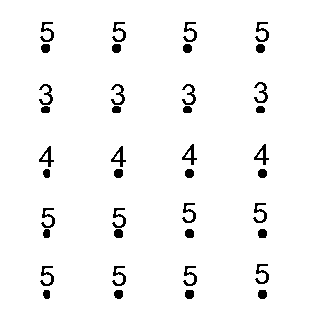
\includegraphics[width=\linewidth]{Images/mu.pdf}
\vspace{-5mm}
\caption{${\mu}$}
\label{fig:mu}
\end{subfigure}
\begin{subfigure}{0.243\linewidth}
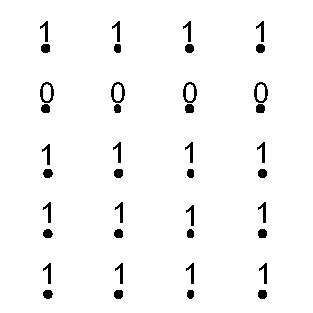
\includegraphics[width=\linewidth]{Images/bvolumeT.pdf}
\vspace{-5mm}
\caption{$bvolume_{T}$}
\label{fig:bvolumeT}
\end{subfigure}
\begin{subfigure}{0.243\linewidth}
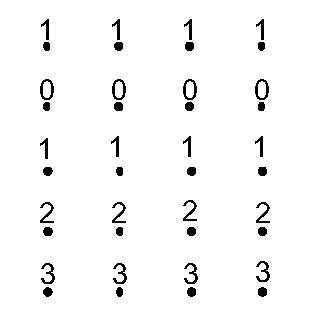
\includegraphics[width=\linewidth]{Images/distanceT.pdf}
\vspace{-5mm}
\caption{$distance_{T}$}
\label{fig:distanceT}
\end{subfigure}
\begin{subfigure}{0.243\linewidth}
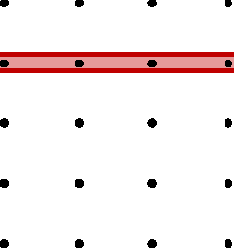
\includegraphics[width=\linewidth]{Images/zlsT.pdf}
\vspace{-5mm}
\caption{$ZLS_{T}$}
\label{fig:zlsT}
\end{subfigure}
\begin{subfigure}{0.243\linewidth}
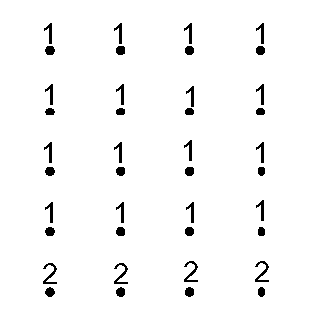
\includegraphics[width=\linewidth]{Images/sigma.pdf}
\vspace{-5mm}
\caption{${\sigma}$}
\label{fig:sigma}
\end{subfigure}
\begin{subfigure}{0.243\linewidth}
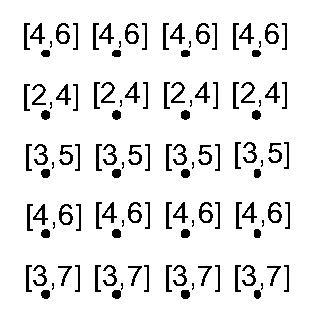
\includegraphics[width=\linewidth]{Images/boundsC.pdf}
\vspace{-5mm}
\caption{$bounds_{C}$}
\label{fig:boundsC}
\end{subfigure}
\begin{subfigure}{0.243\linewidth}
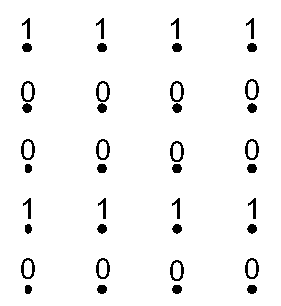
\includegraphics[width=\linewidth]{Images/bvolumeTC.pdf}
\vspace{-5mm}
\caption{$bvolume_{T,C}$}
\label{fig:bvolumeTC}
\end{subfigure}
\begin{subfigure}{0.243\linewidth}
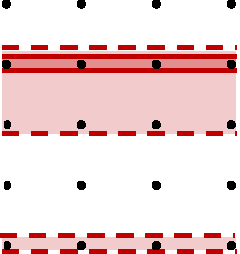
\includegraphics[width=\linewidth]{Images/zlsT_fclsTC.pdf}
\vspace{-5mm}
\caption{{\scriptsize $ZLS_{T}$+$FCLS_{T,C}$}}
\label{fig:fclsTC}
\end{subfigure}
\caption{A notional example showing the steps involved in generating the ``zero'' feature level-set $ZLS_{T}$~(top row) and feature confidence level-set $FCLS_{T,C}$~(bottom row) for an uncertain univariate field represented using ${\mu}$~(a) and ${\sigma}$~(e).
%
For this example, we use trait $T=[2.5, 3.5]$ and confidence $C=68\%$, i.e., $Z=1$.
%
$FCLS_{T,C}$ is computed using the $distance_{T,C}$ (not shown) field.
%
Assuming a unit distance between adjacent grid points,
%
$distance_{T,C}$ would be computed using $bvolume_{T,C}$~(g) as input and would appear equivalent for this example.
%$bvolume_{T,C}$~(g) and $distance_{T,C}$ (not shown) would appear equivalent for this example.
}
\label{fig:example}
\vspace{-5mm}
\end{figure}
